\chapter{Planar graphs}

In this part we are going to focus on one of the most classical (and historical) topics in graph coloring: vertex colorings of planar graphs. 

\begin{definition}
$G$ is \emph{planar} if it can be drawn on ${\rm I\!R^2}$(the plane) so that edges intersect only at their common endpoints.
We call such a drawing an \emph{"embedding"}(some authors say \emph{"drawing"}).
\end{definition}

\begin{example}

\begin {tikzpicture}

\draw   
           node[fill,circle,inner sep=0pt,minimum size=3pt] (n1) at (0,0) {}
	node[fill,circle,inner sep=0pt,minimum size=3pt] (n2) at (1,0) {} 
	node[fill,circle,inner sep=0pt,minimum size=3pt] (n3) at (0,1) {} 
	node[fill,circle,inner sep=0pt,minimum size=3pt] (n4) at (1,1) {}
[line width = 1 pt, black, -] (n1) edge (n4)
[line width = 1 pt, black, -] (n2) edge (n3)
[line width = 1 pt, black, -] (n1) edge (n2)
[line width = 1 pt, black, -] (n2) edge (n4)
[line width = 1 pt, black, -] (n4) edge (n3)
[line width = 1 pt, black, -] (n3) edge (n1)
;
\end{tikzpicture}
       $K_4$ not an embedding
\begin {tikzpicture}
\newcommand*{\OutAngle}{60}
 \newcommand*{\ArcMax}{1.2}
\draw
	node[fill,circle,inner sep=0pt,minimum size=3pt] (n1) at (0,0) {}
	node[fill,circle,inner sep=0pt,minimum size=3pt] (n2) at (1,0) {} 
	node[fill,circle,inner sep=0pt,minimum size=3pt] (n3) at (0,1) {} 
	node[fill,circle,inner sep=0pt,minimum size=3pt] (n4) at (1,1) {}
[line width = 1 pt, black, -] (n1) edge (n2)
[line width = 1 pt, black, -] (n1) edge (n2)
[line width = 1 pt, black, -] (n2) edge (n4)
[line width = 1 pt, black, -] (n4) edge (n3)
[line width = 1 pt, black, -] (n3) edge (n1)
(0, 1) to[out=\OutAngle, in=135]
    (\ArcMax, \ArcMax) to[out=-45, in=90-\OutAngle]
    (1, 0) -- cycle
;
\end{tikzpicture}
embedding ($K_4$ is planar)
\newline
\newline
\begin {tikzpicture}
\draw 
%node[fill,circle,inner sep=0pt,minimum size=3pt] (n1) at (0,0) {}
node[fill,circle,inner sep=0pt,minimum size=3pt] (n2) at (-0.5,0) {}
node[fill,circle,inner sep=0pt,minimum size=3pt] (n3) at (0,0.5) {}
node[fill,circle,inner sep=0pt,minimum size=3pt] (n4) at (0.5,0) {}
node[fill,circle,inner sep=0pt,minimum size=3pt] (n5) at (0,1) {}
[line width = 1 pt, black, -] (n2) edge (n4)
%[line width = 1 pt, black, -] (n1) edge (n4)
[line width = 1 pt, black, -] (n3) edge (n5)
[line width = 1 pt, black, -] (n2) edge (n5)
[line width = 1 pt, black, -] (n4) edge (n5)
[line width = 1 pt, black, -] (n3) edge (n4)
[line width = 1 pt, black, -] (n2) edge (n3)
;
\end{tikzpicture}
straight line-embedding
\end{example}

\begin{theorem}(F{\'a}ry,\emph{1948}) If $G$ has an embedding, then it also has one where every edge is a straight line segment.
\end{theorem}
\begin{remark} $G$ can be treated as a topological space [($CW-$,$\Delta-$,simplicial-) complex]. Then $G$ is planar if (as a topological space) it embeds into ${\rm I\!R^2}$ ($embedding \equiv continuous, injective\ map$)
\end{remark}

\begin{example}
\begin {tikzpicture}
\draw  
	node[fill,circle,inner sep=0pt,minimum size=3pt] (n1) at (0,0) {}
	node[fill,circle,inner sep=0pt,minimum size=3pt] (n2) at (-1,0) {}
	node[fill,circle,inner sep=0pt,minimum size=3pt] (n3) at (1,0) {}
	node[fill,circle,inner sep=0pt,minimum size=3pt] (n4) at (0,-1) {}
	node[fill,circle,inner sep=0pt,minimum size=3pt] (n5) at (-1,-1) {}
	node[fill,circle,inner sep=0pt,minimum size=3pt] (n6) at (1,-1) {}
[line width = 1 pt, black, -] (n2) edge (n5)
[line width = 1 pt, black, -] (n2) edge (n4)
[line width = 1 pt, black, -] (n2) edge (n6)
[line width = 1 pt, black, -] (n1) edge (n5)
[line width = 1 pt, black, -] (n1) edge (n6)
[line width = 1 pt, black, -] (n1) edge (n4)
[line width = 1 pt, black, -] (n3) edge (n4)
[line width = 1 pt, black, -] (n3) edge (n5)
[line width = 1 pt, black, -] (n3) edge (n6);
\end {tikzpicture}
{$K_{3,3}$}
\begin {tikzpicture}
\draw
node[fill,circle,inner sep=0pt,minimum size=3pt] (n1) at (0,0) {}
(0,0) node [text=black,above] {$2$}
node[fill,circle,inner sep=0pt,minimum size=3pt] (n2) at (-1,0) {}
(-1,0) node [text=black,above] {$1$}
node[fill,circle,inner sep=0pt,minimum size=3pt] (n3) at (-1.5,-1) {}
(-1.5,-1) node [text=black,below] {$5$}
node[fill,circle,inner sep=0pt,minimum size=3pt] (n4) at (0.5,-1) {}
(0.5,-1) node [text=black,below] {$3$}
node[fill,circle,inner sep=0pt,minimum size=3pt] (n5) at (-0.5,-1.5) {}
(-0.5,-1.5) node [text=black,below] {$4$}
[line width = 1 pt, black, -] (n2) edge (n5)
[line width = 1 pt, black, -] (n2) edge (n4)
[line width = 1 pt, black, -] (n1) edge (n5)
[line width = 1 pt, black, -] (n3) edge (n5)
[line width = 1 pt, black, -] (n4) edge (n5)
[line width = 1 pt, black, -] (n4) edge (n1)
[line width = 1 pt, black, -] (n1) edge (n2)
[line width = 1 pt, black, -] (n3) edge (n2)
[line width = 1 pt, black, -] (n3) edge (n1)
[line width = 1 pt, black, -] (n3) edge (n4)
[line width = 1 pt, black, -] (n2) edge (n5)
; 
\end {tikzpicture}
{$K_5$}

\end{example}
\bigskip
\bigskip
\begin{observation}\textbf {\textit{"{$K_5$} is not planar"}}
\end {observation}
\begin{proof}
In any planar embedding the cycle 1-2-3-4-5-1 has to be drawn as a polygon: \newline
We can draw at most 2 non intersecting diagonals inside this polygon. \newline
We can draw at most 2 non intersecting diagonals outside this polygon. \newline
\underline {But} we have to draw 5 diagonals, so that is impossible.
\end{proof}

\begin{observation}\textbf {\textit{"{$K_{3,3}$} is not planar"}}
\end{observation}
\begin {proof}
The 6-cycle has to be drawn as a polygon.\newline
We need edges: 15,26,34\newline
At most 1 can appear inside\newline
At most 1 can appear outside
\end {proof}
\begin {tikzpicture}
\draw
node[fill,circle,inner sep=0pt,minimum size=3pt] (n1) at (0,0) {}
	node[fill,circle,inner sep=0pt,minimum size=3pt] (n2) at (-1,0) {}
	node[fill,circle,inner sep=0pt,minimum size=3pt] (n3) at (1,0) {}
	node[fill,circle,inner sep=0pt,minimum size=3pt] (n4) at (0,-1) {}
	node[fill,circle,inner sep=0pt,minimum size=3pt] (n5) at (-1,-1) {}
	node[fill,circle,inner sep=0pt,minimum size=3pt] (n6) at (1,-1) {}
[line width = 1 pt, black, -] (n2) edge (n6)
[line width = 1 pt, black, -] (n1) edge (n5)
[line width = 1 pt, black, -] (n1) edge (n4)
[line width = 1 pt, black, -] (n3) edge (n4)
[line width = 1 pt, black, -] (n3) edge (n6)
[line width = 1 pt, black, -] (n2) edge (n5);
\end {tikzpicture}
{$C_6$}\begin {tikzpicture}
\draw
node[fill,circle,inner sep=0pt,minimum size=3pt] (n1) at (0,0) {}
(0,0) node [text=black,above] {$4$}
node[fill,circle,inner sep=0pt,minimum size=3pt] (n2) at (-1,0) {}
(-1,0) node [text=black,above] {$1$}
node[fill,circle,inner sep=0pt,minimum size=3pt] (n3) at (-1.5,-0.7) {}
(-1.5,-0.7) node [text=black,below] {$6$}
node[fill,circle,inner sep=0pt,minimum size=3pt] (n4) at (0.6,-0.7) {}
(0.6,-0.7) node [text=black,below] {$2$}
node[fill,circle,inner sep=0pt,minimum size=3pt] (n5) at (0,-1.5) {}
(0,-1.5) node [text=black,below] {$5$}
node[fill,circle,inner sep=0pt,minimum size=3pt] (n6) at (-1,-1.5) {}
(-1,-1.5) node [text=black,below] {$3$}
[line width = 1 pt, black, -] (n1) edge node {} (n2)
[line width = 1 pt, black, -] (n1) edge node {} (n4)
[line width = 1 pt, black, -] (n4) edge node {} (n5)
[line width = 1 pt, black, -] (n5) edge node {} (n6)
[line width = 1 pt, black, -] (n6) edge node {} (n3)
[line width = 1 pt, black, -] (n3) edge node {} (n2)
;
\end {tikzpicture}

\begin {definition}\begin{minipage}[t]{\linewidth}
\begin {itemize}
\item An edge subdivision is the replacement 
\begin {tikzpicture}
\draw 
node[fill,circle,inner sep=0pt,minimum size=3pt] (n1) at (0,0) {}
(0,0) node [text=black,above] {$v$}
node[fill,circle,inner sep=0pt,minimum size=3pt] (n2) at (2,0) {}
(2,0) node [text=black,above] {$w$}
[line width = 1 pt, black, -] (n1) edge node {} (n2);
\end {tikzpicture}
\begin {tikzpicture}
\draw 
node[fill,circle,inner sep=0pt,minimum size=3pt] (n1) at (0,0) {}
(0,0) node [text=black,above] {$v$}
[line width = 1 pt, black, -] (n1) edge node {} (n2)
node[fill,circle,inner sep=0pt,minimum size=3pt] (n2) at (1,0) {}
(1,0) node [text=black,above] {$z$}
node[fill,circle,inner sep=0pt,minimum size=3pt] (n3) at (2,0) {}
(2,0) node [text=black,above] {$w$}
[line width = 1 pt, black, -] (n1) edge node {} (n3);
\end {tikzpicture}

where z is a new vertex.
\item An edge contraction is the indentification of the two endpoints of an edge.
\item {H} is minor of {G} if {H} can be obtained from {G} by removing edges and contracting edges.
\end {itemize}
\end {minipage}
\end {definition}

\begin {theorem}The following are equivalent :
\begin{minipage}[t]{\linewidth}
\begin{enumerate}[(a)]
\item {G} is planar
\item {G} contains no iterated subdivision of {$K_5$} or {$K_{3,3}$} as a subgraph 
\newline (Kuratowski,1930)
\item {G} has no {$K_5$} or {$K_{3,3}$} as a minor
\newline (Wagner,1937)
\end {enumerate}
\end {minipage}
\end {theorem}
\bigskip
\begin {example}
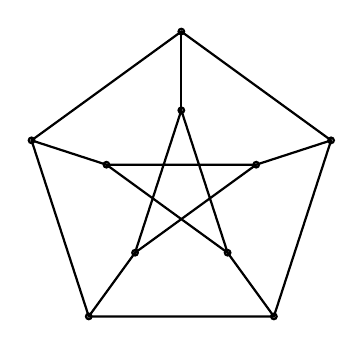
\begin{tikzpicture}[style=thick]
\draw (18:2cm) -- (90:2cm) -- (162:2cm) -- (234:2cm) --
(306:2cm) -- cycle;
\draw (18:1cm) -- (162:1cm) -- (306:1cm) -- (90:1cm) --
(234:1cm) -- cycle;
\foreach \x in {18,90,162,234,306}{
\draw (\x:1cm) -- (\x:2cm);
\draw (\x:2cm) circle (1pt);
\draw (\x:1cm) circle (1pt);
}
\end{tikzpicture}
{$G$}=Petersen graph
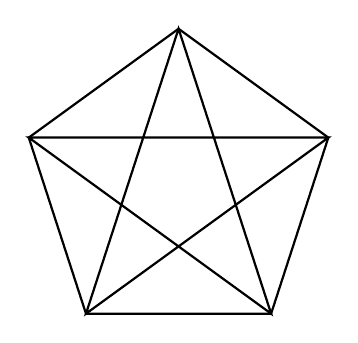
\begin{tikzpicture}[style=thick]
\draw (18:2cm) -- (90:2cm) -- (162:2cm) -- (234:2cm) --
(306:2cm) -- cycle;
\draw (18:2cm) -- (162:2cm) -- (306:2cm) -- (90:2cm) --
(234:2cm) -- cycle;
\foreach \x in {18,90,162,234,306}{}
\end{tikzpicture}
{$K_5$} minor
\end {example}
\begin {remark} If {$G$} is planar then {$G$} has no {$K_5$} or {$K_{3,3}$} subdivision/minor as subgraph
\end {remark}
$(a) \implies (b)$ , $(a) \implies (c)$ are easy implications
\begin {proof} An embedding of {$G$} would contain an embedding of {$K_5$} or {$K_{3,3}$}
\end {proof}
\bigskip
\begin {theorem} (The Four-Color Theorem)
Every planar graph is 4-colorable.
\end {theorem}
\bigskip
\textbf{\textit{Proof history}}
\begin {itemize}
\item 1800-1850 first mentioned
\item 1852 a student of De Morgan conjectured 4-colors are sufficient
\item Cayley popularized it a lot
\item 1879 Alfred Kempe published a proof
\item 1880 Tait had another proof
\item 1890 Heawood found an error in Kempe's proof (but proved the 5-color theorem), 
                  Petersen found an error in Tait's proof
\item 1960 Heesh found a method that could give a proof but involved analysing a huge number of cases
\item 1976 Appel, Haken analysed these cases with a computer ($\approx$ 2000 cases)
\item 1990 Robertson, Seymour and others gave a new computer-assisted proof ($\approx$ 600 cases)
\end {itemize}
\bigskip
\begin {definition} A face is any connected component of ${\rm I\!R^2}$  after removing the embedded graph.
\end {definition}
\begin {observation}\begin{minipage}[t]{\linewidth}
\begin {itemize}
\item There is exactly one unbounded face.
\item Each face is an open subset of ${\rm I\!R^2}$.
\end {itemize}
\end {minipage}
\end {observation}
\begin {observation}
A graph is planar if and only if it can be embedded in ${S^2}$ (the sphere).
Suppose {$G$} is embedded in ${S^2}$.Pick a point of ${S^2}$ not in the embedding.
Use the stereographic projection to map {$G$} onto ${\rm I\!R^2}$.
Note that in a spherical embedding each face is bounded and homeomorphic to an open disk.
\end {observation}
\bigskip
\bigskip
\begin {example} {$Q_3$} as planar graph.
\begin{tikzpicture}[style=thick]
\draw (0,0) -- (2,0) -- (2,2) -- (0,2) -- (0,0)
(0.5,0.5) -- (1.5,0.5) -- (1.5,1.5) -- (0.5,1.5) -- (0.5,0.5)
(0.5,0.5) -- (0,0)
(1.5,0.5) -- (2,0)
(1.5,1.5) -- (2,2)
(0.5,1.5) -- (0,2);
\end {tikzpicture}
\end {example}
\bigskip
\underline{\textbf{Notation}} Suppose I have {$G$} with a fixed planar embedding (or spherical embedding)
\newline
				     {$v$}= \# vertices, {$e$}= \# edges, {$f$}= \# faces.
\begin {theorem}
(Euler's formula) If G is planar and connected, then for any planar embedding of {$G$} :   
$$v-e+f=2.$$
\end {theorem}
\begin {proof}
By induction
\newline
If {$f$}={$1$} then {$G$} has no cycles, as otherwise any cycle of the graph would seperate ${\rm I\!R^2}$ into at $\geq 2$ parts. Hence {$G$} is a tree, $e=v-1$ and
$$v-e+f=v-(v-1)+1=2.$$
If $f\geqslant 2$ then pick an edge $xy\in E(G)$ so that on the two sides of {$xy$} we have two different faces of the embedding.
Now {$G-xy$} is planar, connected and it has 
{$f(G-xy)$}={$f(G)-1$},
{$e(G-xy)$}={$e(G)-1$},
{$v(G-xy)$}={$v(G)$}. 
The proof follows by induction.
\end {proof}
\bigskip
Euler cared about regular polyhedra in ${\rm I\!R^3}$
\newline
\underline{\textbf{Very quick application}}: Classification of Platonic solids (regular polytopes).
\begin {definition} A polytope is regular if:
\begin {enumerate}
\item All vertices have the same degree $k\geqslant3$,
\item All faces are polygons with the same number of sides $l\geqslant3$.
\end {enumerate}
\end {definition}
Let it have {$v$} vertices, {$e$} edges, {$f$} faces in the spherical embedding.

We have these equations:
$\begin{cases}
v-e+f=2\\
kv=2e \\
lf=2e 
\end {cases}$

and so:

$e(\frac{2}{k}-1+\frac{2}{l})=2 \implies \frac{2}{k}+\frac{2}{l}=1+\frac{2}{e}\implies \frac{1}{k}+\frac{1}{l}=\frac{1}{2}+\frac{2}{e}\textgreater \frac{1}{2}$. 

This can be satisfied only for $(k,l)=(3,3),(3,4),(3,5),(4,3),(5,3)$. For each case we uniquely determine $v,e,f$.

\begin{corollary}\begin{minipage}[t]{\linewidth}
Suppose $G$ has at least three vertices.
\begin {enumerate}[(a)]
\item If {$G$} is planar then $e\leqslant3v-6$
\item  If {$G$} is planar and triangle free then $e\leqslant2v-4$
\end {enumerate}
\end {minipage}
\end {corollary}
\begin {proof} We can assume {$G$} is connected. Then $v-e+f=2$.
Count the edges around each face. Each face has length $\geqslant3$ so we get at least ${3f}$.
But each edge is counted twice, so we get exactly $2e$. That means 
$2e\geqslant3f$ or $f\leqslant\frac{2}{3}e$.
\newline
$2=v-e+f\leqslant v-e+ \frac{2}{3}e=v- \frac{1}{3}e$
\newline
$e\leqslant 3v-6$
\newline
If {$G$} is triangle-free then we have a stronger inequality
$2e\geqslant 4f$
and continue the same way.
\end {proof}
\begin {observation} This gives another proof of non-planarity of {$K_{3,3}$} and {$K_5$}
\newline
{$K_5$}: $v=5,e=10$    \: \:\:\:\:\: $10\nleq3\cdot5-6$
\newline
{$K_{3,3}$}: is triangle-free, $v=6, e=9 \: \: \: \: 9\nleq2\cdot6-4$
\end {observation}





\begin{theorem}[5-color theorem]
If $G$ is planar then $\chi(G) \leq 5$.
\end{theorem}
\begin{proof}
Later: "Proof from the book" (Aigner, Zeigler).
\end{proof}

List coloring, examples:
\begin{itemize}
\item[1]A graph $G(V,E)$ with
	\begin{itemize}
	\item V = courses
	\item E = conflicts (student in both courses)
	\end{itemize}
	can be subject to a list-coloring should there restrictions to for instance  the choices of days that a course can be held at. 
\item[2]Soduku $\equiv$ coloring of $9\times 9$ grid with restrictions in the form of already given numbers.
\end{itemize}

As a definition:
\begin{definition}
Let $G$ be any graph, for every vertex $x\in V(G)$ we have a set of colors $L(x)$ ( of colors available to $x$).

A $L$-coloring of $G$ is a coloring $c:V(G)\rightarrow \underset{x}{\bigcup} L(x)$ such that $c(x)\in L(x)$ for all $x$. 

The list-chromatic number $\chi_{\ell}(G)$ is the smallest $k$ s.t. $G$ has a $L$-coloring for any choice of list satisfying $|L(x)|\geq k$. 

$G$ is $k$-list-colorable ($k$-choosable) when $\chi_{\ell}(G)\leq k$.
\end{definition}

\begin{example}
Here are some various examples and facts:

\begin{itemize}
\item $L(x)=\{1,\ldots,k\}$ for all $x\in V(G)$ then $L$-coloring $\equiv$ $k$-coloring in the normal sense
\item $\chi(G)\leq \chi_{\ell}(G)$
\item Example with $\chi(G) < \chi_{\ell}(G)$:
\begin{center}
\begin{tikzpicture}[
every node/.style={circle,inner sep=2pt,fill,draw}
]
\node[label={[label distance=1pt]90:$2,3$}] (A) at (-2,1) {};
\node[label={[label distance=1pt]90:$1,2$}] (B) at (0,1) {};
\node[label={[label distance=1pt]90:$1,3$}] (C) at (2,1) {};

\node[label={[label distance=1pt]270:$1,3$}] (D) at (-1,-1) {};
\node[label={[label distance=1pt]270:$1,2$}] (E) at (1,-1) {};
\node[label={[label distance=1pt]270:$2,3$}] (F) at (3,-1) {};

\draw[thick] (A) -- (D);
\draw[thick] (A) -- (E) ;

\draw[thick] (B) -- (D);
\draw[thick] (B) -- (F);
\draw[thick] (B) -- (E);

\draw[thick] (C) -- (E);
\draw[thick] (C) -- (F);

\end{tikzpicture}
\end{center}
For each $x$, $|L(x)|=2$. But for these list there are no $L$-coloring. Therefore $\chi_{\ell}(G)\geq 3$, while $\chi(G)=2$ since the graph is bipartite.
\item $\chi_{\ell}(G)\leq \Delta G+1$, same proof as the non-list chromatic number.
\item Brooks Theorem holds.
\end{itemize}
\end{example}

\textbf{Question:} Can we construct $G$ with small $\chi(G)$ and large $\chi_{\ell}(G)$?

\begin{proposition}
For every $k\geq 2$ there exist a graph with $\chi(G)=2$ and $\chi_{\ell}(G)>k$
\end{proposition}

\begin{proof}
Take $A=B=\binom{\{1,\ldots,2k-1\}}{k}$, (the set of all $k$-subsets of $\{1,\ldots,2k-1\}$).

Let $G=K_{A,B}$ be the complete bipartite graph with parts $A$ and $B$.
\begin{example}
Take $k=3, |A|=|B|=\binom{5}{3}=10$

That is $A$ and $B$ will consist of 10 vertices each with a list of three numbers made of the various permutations of $[1,2,3,4,5]$ and every vertex in $A$ is connected to every vertex in $B$. So $|V|=20, |E|=100$.
\end{example}

(\textit{proof} cont.)
For $X \in A$ or $X \in B$ set $L(X)=X$ and note $|L(X)|=k.$
We claim that $K_{A,B}$ has no $L$-coloring.

Suppose $c$ is an $L$-coloring. Then $c(A)\subseteq \{1,\ldots,2k-1\}$, $|c(A)|\geq k$. $\leftarrow$ will be true, or otherwise $|c(A)|\leq k-1$ and then there is a $X\subseteq\{1,\ldots,2k-1\}$ such that $|X|=k$ and $X\cap c(A)=\emptyset$. Then $X$ cannot be colored with a color from $L(X)$.

Similar for $B$, that is  $c(B)\subseteq \{1,\ldots,2k-1\}$, $|c(B)|\geq k$.

It follows  that $c(A)\cap c(B)\neq \emptyset$ so two vertices on opposite sides have the same color. That means $\chi_{\ell}(K_{A,B})\geq k+1$, but $\chi(K_{A,B})=2$.
\end{proof}

\begin{theorem}
(Thomassen 1994)

Every planar graph satisfies $\chi_{\ell}(G)\leq 5$. (It is 5-list-colorable).  
\end{theorem}
\begin{remark}
This is stronger than the 5-color theorem, because $\chi(G)\leq \chi_{\ell}(G)$.
\end{remark}

\begin{definition}
An embedding of a planar graph $G$ is called:
\begin{itemize}
\item A triangulation if every face is a triangle (also the unbounded one)
\item A near-triangulation if every bounded face is a triangle and the unbounded one is a cycle.
\end{itemize}
\end{definition}

\begin{example}
Various examples of Definition 8.
\begin{center}
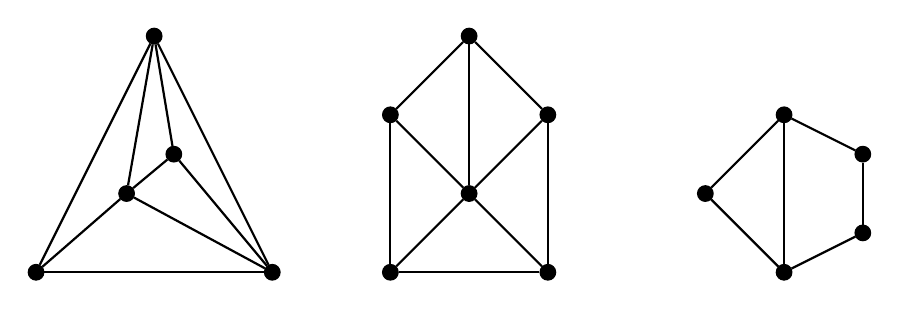
\begin{tikzpicture}[
every node/.style={circle,inner sep=2pt,fill,draw}
]
\node (a) at (-5,2) {};
\node (b) at (-5.35,0) {};
\node (c) at (-4.75,0.5) {};
\node (d) at (-6.5,-1) {};
\node (e) at (-3.5,-1) {};

\draw[thick] (a) -- (b);
\draw[thick] (a) -- (c) ;
\draw[thick] (a) -- (d);
\draw[thick] (a) -- (e);
\draw[thick] (b) -- (c);
\draw[thick] (b) -- (d);
\draw[thick] (b) -- (e);
\draw[thick] (d) -- (e);
\draw[thick] (c) -- (e);

\node (f) at (-2,-1) {};
\node (g) at (-2,1) {};
\node (h) at (-1,0) {};
\node (i) at (-1,2) {};
\node (j) at (0,-1) {};
\node (k) at (0,1) {};

\draw[thick] (f) -- (g);
\draw[thick] (g) -- (i);
\draw[thick] (i) -- (k);
\draw[thick] (j) -- (k);
\draw[thick] (j) -- (f);
\draw[thick] (h) -- (f);
\draw[thick] (h) -- (g);
\draw[thick] (h) -- (i);
\draw[thick] (h) -- (k);
\draw[thick] (h) -- (j);

\node (l) at (2,0) {};
\node (m) at (3,1) {};
\node (n) at (3,-1) {};
\node (o) at (4,0.5) {};
\node (p) at (4,-0.5) {};

\draw[thick] (l) -- (m);
\draw[thick] (m) -- (o);
\draw[thick] (o) -- (p);
\draw[thick] (p) -- (n);
\draw[thick] (n) -- (l);
\draw[thick] (n) -- (m);

\end{tikzpicture}
\end{center}
From left to right: A triangulation, a near triangulation and the final picture is neither.
\end{example}

\begin{remark}
Every embedding can be extended to a triangulation on the same vertex set. (By only adding edges)
\end{remark}
\begin{proof}
Add diagonals as needed. It also work for the unbounded face.
\end{proof} 

In other words:
For any planar $G$ there is a triangulation $H$ such that
\begin{align*}
V(G)=V(H), \ E(G)\subseteq E(H).
\end{align*} 
In particular
\begin{align*}
\chi(G) &\leq \chi(H)
\\
\chi_{\ell}(G) &\leq \chi_{\ell}(H)
\end{align*}

\begin{proposition}
Suppose $G$ is near-triangular with outer cycle $\mathbb{O}=x_1,\ldots,x_k$ and assume the following exist:
\begin{itemize}
\item $L(x_1)=\{a\}$, $L(x_2)=\{b\}$, $a\neq b$
\item $|L(x_i)|\geq 3$ for all $i=3,\ldots,k-1$
\item $|L(y)|\geq 5$ for all $y\notin \mathbb{O}$.
\end{itemize}
Then $G$ is L-colorable.
\end{proposition}

\begin{remark}
This proposition implies Thomassens theorem as follows:

Take $H$, any planar graph, with lists $L$ and $|L(x)| \geq 5$. Extend $H$ to a triangulation $H\subseteq G$ (in particular, $G$ is a near-triangulation). Choose any $x_1,x_2$ on the outer face. Restrict $L(x_1)$ and $L(x_2)$ to one element and voila! $\rightarrow$ the proposition applies to $G$. 

$L$-coloring of $G$ gives an $L$-coloring for $H$.
\end{remark}

\begin{proof}
Proof of proposition 11:

\begin{itemize}
\item $|V(G)|=3$: 
\begin{center}
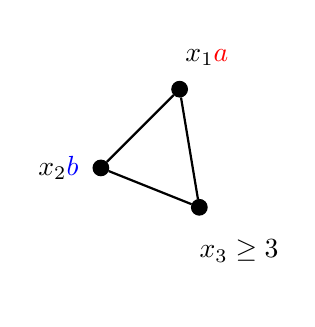
\begin{tikzpicture}[
every node/.style={circle,inner sep=2pt,fill,draw}
]
\node[label={[label distance=1pt]60:$x_1 {\color{red}a}$}] (A) at (1,1) {};
\node[label={[label distance=1pt]180:$x_2 {\color{blue}b}$}] (B) at (0,0) {};
\node[label={[label distance=1pt]300:$x_3 \geq 3$}] (C) at (1.25,-0.5) {};


\draw[thick] (A) -- (B);
\draw[thick] (A) -- (C) ;
\draw[thick] (B) -- (C);

\end{tikzpicture}
\end{center}
Then we will have a spare color for $x_3$.
\end{itemize}

\underline{Case 1}:

There is an edge $x_k x_j$, $j=2,\ldots,k-2$
\begin{center}
\includegraphics[scale=0.25]{Case1}
\end{center}
\begin{itemize}
\item[•]$G_1=$ graph bounded by $x_1x_2\ldots x_jx_k \rightarrow$ $L$-color $G_1$ by induction.
\item[•] $G_2=$ graph bounded by $x_kx_j\ldots x_{k-1} \rightarrow $ $L$-color $G_2$ by induction.
\item[•] $\rightarrow$ L-coloring of $G$. Note that after coloring $G_1$ some colors are not available for certain vertices of $G_2$, but there is enough left just to use the induction hypothesis for $G_2$.
\end{itemize}

\underline{Case 2}:

There are no edge $x_k x_j$, $j=2,\ldots,k-2$.
\begin{itemize}
\item Around $x_k$ we must have a sequence of triangles, since the interior is triangulated.
\item Let $N(X_k)=\{x_1,x_{k-1},y_1,\ldots,y_{\ell}\}$
\item Pick $c,d \in L(X_k)$, $c\neq d$, $c,d \neq a$.
\item Set $G'=G-x_k$ and note that $G' $ is a near-triangulation. 
\end{itemize}
\begin{center}
\includegraphics[scale=0.125]{Case2}
\end{center}
Consider the list:
\begin{align*}
L'(y_i)=L(y_i)\backslash \{c,d\} \ , \ L'(x)=L(x) \ \text{for any other} \ x \in G'
\end{align*}
$\leadsto$ There is a L'-coloring of $G'$ by induction.
\begin{align*}
c(y_i)\notin \{c,d\} \ , \ c(x_1) \notin \{c,d\}
\end{align*}
$\leadsto$ color $x_k$ with either $c$ or $d$ depending on $c(x_{k-1})$.
\end{proof}

\begin{remark}
There are planar not-4-list-colorable graphs. (Voigt '93 example with $\approx$ 300 vertices).
\end{remark}
\begin{remark}
Did not use Euler, upper/lower bounds. Only geometric properties.
\end{remark}
\subsubsection*{Application:
\underline{The art gallery problem}}

Suppose $P$ is a polygon in $\mathbb{R}^2$ with $n$ vertices.

\begin{example}
:
\begin{center}
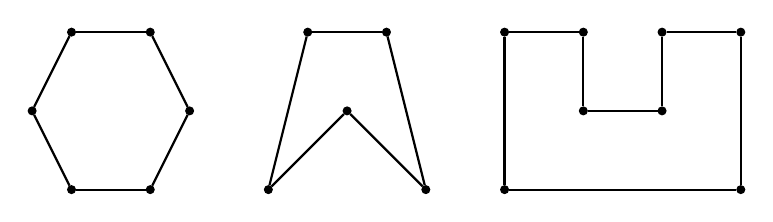
\begin{tikzpicture}[
every node/.style={circle,inner sep=1pt,fill,draw}
]
\node (a) at (-4,0) {};
\node (b) at (-3.5,1) {};
\node (c) at (-3.5,-1) {};
\node (d) at (-2.5,1) {};
\node (e) at (-2.5,-1) {};
\node (f) at (-2,0) {};

\draw[thick] (a) -- (b);
\draw[thick] (a) -- (c) ;
\draw[thick] (b) -- (d);
\draw[thick] (d) -- (f);
\draw[thick] (e) -- (f);
\draw[thick] (e) -- (c);

\node (g) at (-1,-1) {};
\node (h) at (-0.5,1) {};
\node (i) at (0,0) {};
\node (j) at (0.5,1) {};
\node (k) at (1,-1) {};

\draw[thick] (h) -- (g);
\draw[thick] (g) -- (i);
\draw[thick] (h) -- (j);
\draw[thick] (j) -- (k);
\draw[thick] (k) -- (i);

\node (l) at (2,-1) {};
\node (m) at (2,1) {};
\node (o) at (3,1) {};
\node (p) at (3,0) {};
\node (q) at (4,0) {};
\node (r) at (4,1) {};
\node (s) at (5,1) {};
\node (t) at (5,-1) {};

\draw[thick] (l) -- (m);
\draw[thick] (m) -- (o);
\draw[thick] (o) -- (p);
\draw[thick] (p) -- (q);
\draw[thick] (q) -- (r);
\draw[thick] (r) -- (s);
\draw[thick] (s) -- (t);
\draw[thick] (t) -- (l);


\end{tikzpicture}
\end{center}

\end{example}

We assume the bounded region is the floor plan af an art gallery.
\begin{quote}
How many guards are needed to guard each point in sight?
\end{quote}

\begin{problem}
\begin{itemize}
\item Find a gallery with 6 vertices requiring $\geq 2$ guards.
\item Find a gallery with as few vertices as possible requiring $\geq k$ guards.
\end{itemize}
\end{problem}

\begin{observation}
There are $n$-vertex galleries requiring at least $\left \lfloor \frac{n}{3} \right \rfloor$ guards.
\end{observation}
\begin{center}
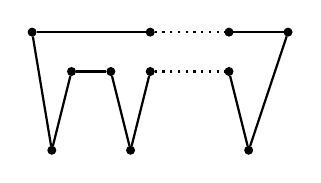
\begin{tikzpicture}[
every node/.style={circle,inner sep=1pt,fill,draw}
]
\node (a) at (-3.5,1.5) {};
\node (b) at (-3.25,0) {};
\node (c) at (-3,1) {};
\node (d) at (-2.5,1) {};
\node (e) at (-2.25,0) {};
\node (f) at (-2,1) {};
\node (g) at (-1,1) {};
\node (h) at (-0.75,0) {};
\node (i) at (-0.25,1.5) {};
\node (f') at (-2,1.5) {};
\node (g') at (-1,1.5) {};

\draw[thick] (a) -- (b);
\draw[thick] (b) -- (c) ;
\draw[thick] (c) -- (d);
\draw[thick] (d) -- (e);
\draw[thick] (e) -- (f);
\draw[dotted, thick] (f) -- (g);
\draw[thick] (g) -- (h);
\draw[thick] (h) -- (i);
\draw[dotted, thick] (f') -- (g');
\draw[thick] (i) -- (g');
\draw[thick] (a) -- (f');

\end{tikzpicture}
\end{center}

\begin{theorem}
Rephrasing the art gallery problem:

Every n-vertex gallery can be guarded by $\left \lfloor \frac{n}{3} \right \rfloor$ guards. ($\approx$ 70's Chvatal).
\end{theorem}

\begin{definition}
A planar embedding is called a \emph{polygon triangulation} if it is a near-triangulation and all vertices lie on the outer cycle.
\end{definition}

\begin{example}
"Polygon triangulated by diagonals"
\begin{center}
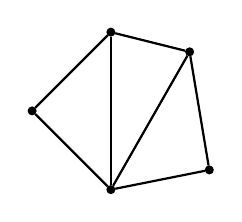
\begin{tikzpicture}[
every node/.style={circle,inner sep=1pt,fill,draw}
]
\node (a) at (-1,0) {};
\node (b) at (0,1) {};
\node (c) at (0,-1) {};
\node (d) at (1,0.75) {};
\node (e) at (1.25,-0.75) {};

\draw[thick] (a) -- (b);
\draw[thick] (a) -- (c);
\draw[thick] (c) -- (b);
\draw[thick] (d) -- (c);
\draw[thick] (b) -- (d);
\draw[thick] (c) -- (e);
\draw[thick] (d) -- (e);

\end{tikzpicture}
\end{center}
\end{example}

\begin{observation}
A triangulated polygon with n vertices has $2n-3$ edges, $n$ on the outer cycle and $n-3$ diagonals.
\end{observation}

\begin{observation}
Every triangulated polygon have a vertex of degree 2.
\end{observation}
\begin{proof}
The shortest diagonal cuts off such a vertex.
\end{proof}

\begin{observation}
Every triangulated polygon is 3-colorable.
\end{observation}
\begin{proof}
Take $v$ to be a vertex of degree 2. $G-v$ is a triangulated polygon. Color $G-v$ with 3 colors, the neighbours of $v$ will use 2 colors. Color $v$ with the spare color.
\end{proof}

\begin{proof}
Proof of Theorem 18:

\begin{itemize}
\item Let $G$ be planar polygon with $n$ vertices.
\item First triangulate using diagonals (Exercise: show that this is always possible).
\item The resulting triangular polygon is 3-colorable. 
\item Some color class will have $\leq \left \lfloor \frac{n}{3} \right \rfloor$ elements
\item Place guards at the vertices of that color.
\end{itemize}
\end{proof}
%%%%%%%%%%%%%%%%%%%%%%%%%%%%%%%%%%%%%%%%
